% --------------------------------------------------------------
%     DENNE MALEN ER LAGET AV MARTIN SORIA RØVANG
%     TIL BRUK FOR OPPGAVELØSNINGER OG RAPPPRTER
%     GITHUB: github.com/martinrovang
% --------------------------------------------------------------


\documentclass[10pt]{article}
\usepackage{amsmath,amsthm,amssymb}
\usepackage{float}
\usepackage[norsk]{babel}
\usepackage[table]{xcolor}
\usepackage{color}
\usepackage{graphicx}
\usepackage{listings}
\usepackage{natbib}
\usepackage[utf8]{inputenc}
\usepackage{imakeidx}
\usepackage[a4paper]{geometry}
\usepackage[myheadings]{fullpage}
\usepackage{fancyhdr}
\usepackage{lastpage}
\usepackage{graphicx, wrapfig, subcaption, setspace, booktabs}
\usepackage[T1]{fontenc}
\usepackage[font=small, labelfont=bf]{caption}
\usepackage{fourier}
\usepackage[protrusion=true, expansion=true]{microtype}
\usepackage{url, lipsum}
\usepackage{tgbonum}
\usepackage{hyperref}
\usepackage{xcolor}
\usepackage[most]{tcolorbox}
\usepackage{mathtools}
\usepackage[page]{totalcount}
\usepackage{lastpage}


\newcommand{\HRule}[1]{\rule{\linewidth}{#1}}
\onehalfspacing
\setcounter{tocdepth}{5}
\setcounter{secnumdepth}{5}
\newcommand{\vect}[1]{\boldsymbol{#1}}

\definecolor{codegreen}{rgb}{0,0.6,0}
\definecolor{codegray}{rgb}{0.5,0.5,0.5}
\definecolor{codepurple}{rgb}{0.58,0,0.82}
\definecolor{backcolour}{rgb}{0.95,0.95,0.92}
\definecolor{skyblue}{rgb}{0.950, 1, 1}

\lstdefinestyle{mystyle}{
    backgroundcolor=\color{backcolour},   
    commentstyle=\color{codegreen},
    keywordstyle=\color{magenta},
    numberstyle=\tiny\color{codegray},
    stringstyle=\color{codepurple},
    basicstyle=\footnotesize,
    breakatwhitespace=false,         
    breaklines=true,                 
    captionpos=b,                    
    keepspaces=true,                 
    numbers=left,                    
    numbersep=5pt,                  
    showspaces=false,                
    showstringspaces=false,
    showtabs=false,                  
    tabsize=2,
    frame=single,
    %keywordstyle=\color{blue},
    language=Python,
    backgroundcolor = \color{skyblue}
}
 
\lstset{style=mystyle}
\lstset{
    basicstyle=\footnotesize\ttfamily,
  identifierstyle=\bfseries\color{green!40!black},
  commentstyle=\itshape\color{purple!40!black},
  keywordstyle=\color{blue},
  stringstyle=\color{orange},
}

\newcommand{\N}{\mathbb{N}}
\newcommand{\Z}{\mathbb{Z}}
 
\newenvironment{theorem}[2][Theorem]{\begin{trivlist}
\item[\hskip \labelsep {\bfseries #1}\hskip \labelsep {\bfseries #2.}]}{\end{trivlist}}
\newenvironment{lemma}[2][Lemma]{\begin{trivlist}
\item[\hskip \labelsep {\bfseries #1}\hskip \labelsep {\bfseries #2.}]}{\end{trivlist}}
\newenvironment{exercise}[2][Exercise]{\begin{trivlist}
\item[\hskip \labelsep {\bfseries #1}\hskip \labelsep {\bfseries #2.}]}{\end{trivlist}}
\newenvironment{problem}[2][Problem]{\begin{trivlist}
\item[\hskip \labelsep {\bfseries #1}\hskip \labelsep {\bfseries #2.}]}{\end{trivlist}}
\newenvironment{question}[2][Question]{\begin{trivlist}
\item[\hskip \labelsep {\bfseries #1}\hskip \labelsep {\bfseries #2.}]}{\end{trivlist}}
\newenvironment{corollary}[2][Corollary]{\begin{trivlist}
\item[\hskip \labelsep {\bfseries #1}\hskip \labelsep {\bfseries #2.}]}{\end{trivlist}}

\newenvironment{solution}{\begin{proof}[Solution]}{\end{proof}}
    
\makeindex[columns=3, title=Alphabetical Index, intoc]


% --------------------------------------------------------------
%                         Headers and footers
% --------------------------------------------------------------
\fancyhf{}
\pagestyle{fancy}
\rhead{Martin Soria Røvang}
\lhead{STA-2003-Tidsrekker}
\rfoot{Side \thepage \, av \pageref{LastPage}}
\renewcommand{\headrulewidth}{0.3pt}
\usepackage{gensymb}
\usepackage{amsmath}
\usepackage{amsfonts}
\usepackage[section]{placeins}


\begin{document}
% --------------------------------------------------------------
%                         FRONTPAGE
% --------------------------------------------------------------
{\fontfamily{cmr}\selectfont
\title{ \normalsize \textsc{}
		\\ [1.0cm] % How much upper margin
		%\HRule{0.5pt} \\
        \LARGE \textbf{\uppercase{Obligatorisk Oppgave 3}
        \HRule{0.5pt} \\ [0.5cm]
        STA-2003-Tidsrekker
        %\HRule{2pt} \\ [0.5cm]
        \\
		\normalsize \today \vspace*{5\baselineskip}}
		}

        \date{}
\author{
		Martin Soria Røvang \\ 
        Universitetet i Tromsø\\}

% \begin{titlepage}
\clearpage\maketitle
\vspace{0.2\textheight}
{\centering
Inneholder \pageref{LastPage} \, sider, inkludert forside.\par
}}
\thispagestyle{empty}
% \end{titlepage}

\newpage
\tableofcontents
% --------------------------------------------------------------
%                         Start here
% --------------------------------------------------------------

% \cite{alpaydin_2014}
\newpage

\section{Oppgave}
\subsection{a)}

Ved bruk av en vektet periodogram vist i ligning(\ref{vektet periodogram}) kan vi se på energien til tidsrekken. Denne viser at vi har kraftig periode rundt $f = 0.5$ år og på $f = 1$ år, derfor kan man se at det er sesongvariasjoner i tidsrekken.

\begin{equation}
    S_{xx}(f) = \frac{dt}{NU}\bigg |\mathfrak{F}\bigg\{w[n]\cdot x[n]\bigg\}\bigg |^{2}
    \label{vektet periodogram}
\end{equation}

Her er $S_{xx}$ kraften på frekvenskomponentene, dt er tidssteget (i dette tilfelle dt = 1), $\mathfrak{F}$ er Fouriertransformasjonen, $w[n]$ er vinduet (brukt hann vindu) og $x[n]$ er tidsrekken. Resultatet er i figur(\ref{task_a}).

\begin{figure}[hbt!]
{\centering
    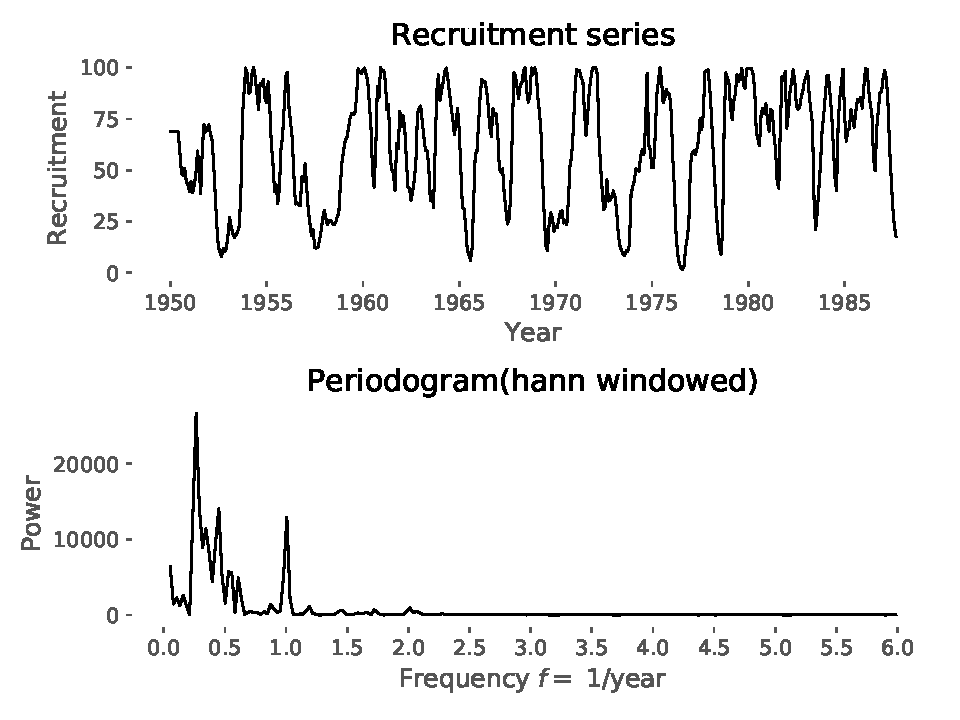
\includegraphics[width=0.70\textwidth]{task_a.pdf}
    \caption{Tidsrekken plottet med vektet periodogram. Her kan man se forskjellige periodisiteter rundt f = 0.5 år og en på f = 1 år. Frekvensaksen har blitt ganget med [12 måneder/år] for å få enhet 1/år.}
    \label{task_a}
\par}
\end{figure}


\subsection{b)}

Her trekker vi fra midlere sesongvariasjoner for å gjøre tidsrekken stasjonær. Resultatet er plottet i figur(\ref{task_b}).

\begin{figure}[hbt!]
    {\centering
        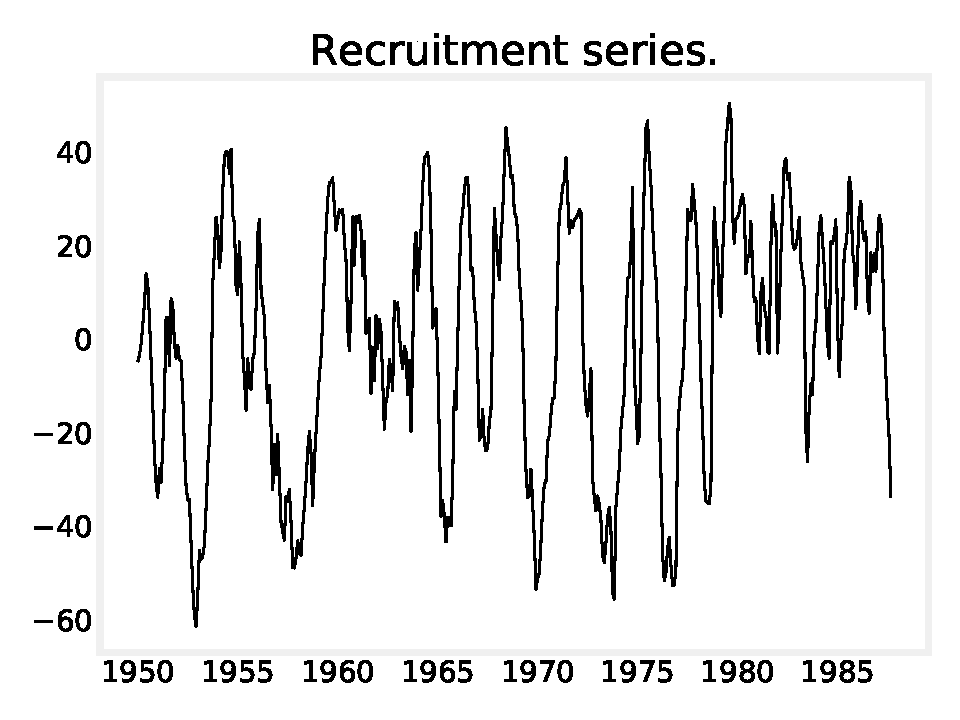
\includegraphics[width=0.70\textwidth]{task_b.pdf}
        \caption{Trukket fra midlere sesongvariasjoner for å gjøre tidsrekken stasjonær.}
        \label{task_b}
    \par}
    \end{figure}


\subsection{c-d)}

Vi har plott av ACF og PACF i figur(\ref{task_c}). Her kan man observere at ACF plottet har den karakteristiske AR() modellen der det konvergerer mot null når $h \rightarrow 0$, men denne gir ingen indikasjon på orden av AR. I PACF ser man at det er en korrelasjon ved $h = 1$ og $h = 2$, resten ser ut til å være hvit støy da dette ligger under 95\% konfidensinterval gitt i ligning(\ref{whitenoiseCI}). Pågrunn av den klare indikatoren på korrelasjon ved $h = 1$ og $h = 2$ kan vi si at vi har en AR(2) eller ARMA(2, 0) prosess. 

\begin{equation}
    \sigma_{w} = \frac{2}{\sqrt{N}}
\label{whitenoiseCI}
\end{equation}
N er lengden på tidsserien.[p. 31 \cite{Timeseries}]


\begin{figure}[hbt!]
    {\centering
        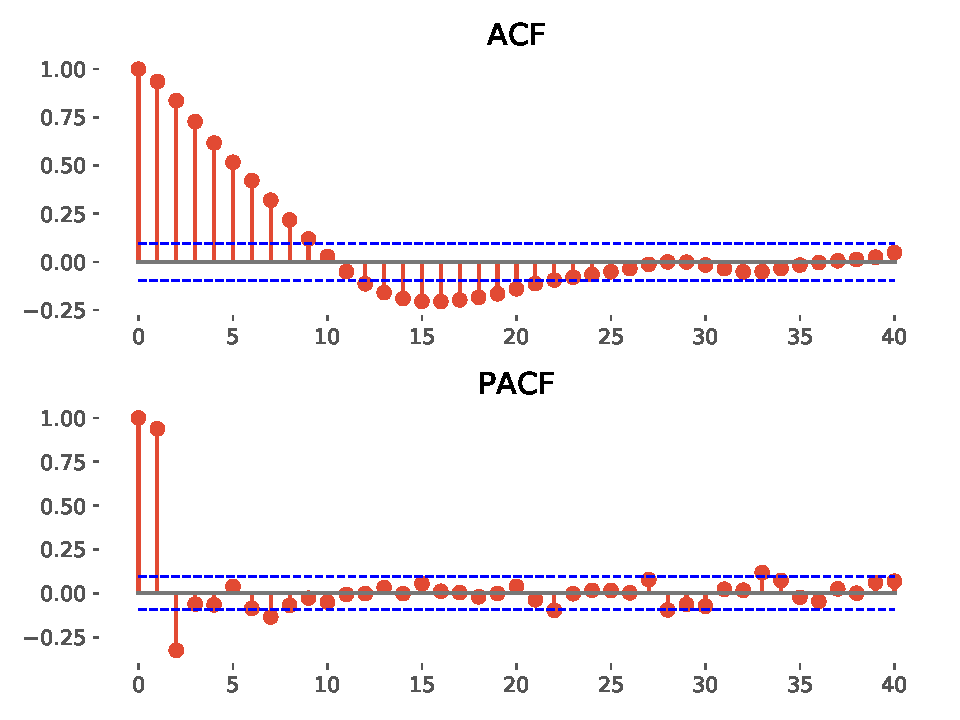
\includegraphics[width=0.70\textwidth]{task_c.pdf}
        \caption{Plot av ACF og PACF for den stasjonære tidsrekken i figur(\ref{task_b})}
        \label{task_c}
    \par}
    \end{figure}




\subsection{e)}
Ved bruk av statsmodels-pakken i python kan vi simulere en ARMA-modell med gitte parametere, i figur(\ref{Armacoefs}) ser vi en resultatet fra en ARMA(2,0) modell. Fra utskriften fikk vi modellen gitt i ligning()

\begin{equation}
\hat{x}_{n} = \alpha + \phi_{1}\hat{x}_{n-1} + \phi_{2}\hat{x}_{n-2} + \hat{w}_{t}
\end{equation}

der $\alpha = -0.7019$, $\phi_{1} = 1.2483$ og $\phi_{2} = -0.3313$
Her har det blitt brukt en \emph{hatt} på tidsrekken for å vise at det er et estimat. Fra utskriften i figur(\ref{Armacoefs}) har vi at $\sigma_{w} = 8.653$, dette er den estimerte variansen på den hvite støyen slik man har fordelingen $N \thicksim (0, \sigma_{w}^{2})$. Dette kan brukes til å finne \emph{Mean-square prediction error} som er gitt ved ligning(\ref{mean-square-predictor-error}),

\begin{equation}
    P^{n}_{n + m} = E\bigg[\sigma_{w}^{2}\sum_{j = 0}^{m-1}\psi_{j}^{2}\bigg]
    \label{mean-square-predictor-error}
\end{equation}

der $\psi$ er vektene gitt fra modellen slik at $\phi(z)\psi(z) = \theta(z)$. Her er $\psi(z)$ og $\theta(z)$ de karakteristiske ligningene til AR og MA modellen og $\psi(z)$ er vektene gitt ved $\psi(z) = (1 + \psi_{1}z + \psi_{2}z^2 + \cdots + \psi_{j}z^{j}+\cdots)$

\begin{figure}[hbt!]
    \begin{lstlisting}
                                    ARMA Model Results
        ==============================================================================
        Dep. Variable:                      y   No. Observations:                  453
        Model:                     ARMA(2, 0)   Log Likelihood               -1616.790
        Method:                       css-mle   S.D. of innovations              8.564
        Date:                Tue, 16 Apr 2019   AIC                           3241.579
        Time:                        12:27:46   BIC                           3258.043
        Sample:                             0   HQIC                          3248.066
        
        ==============================================================================
                         coef    std err          z      P>|z|      [0.025      0.975]
        ------------------------------------------------------------------------------
        const         -0.7019      4.773     -0.147      0.883     -10.057       8.653
        ar.L1.y        1.2483      0.044     28.159      0.000       1.161       1.335
        ar.L2.y       -0.3313      0.044     -7.471      0.000      -0.418      -0.244
                                            Roots
        =============================================================================
                          Real          Imaginary           Modulus         Frequency
        -----------------------------------------------------------------------------
        AR.1            1.1555           +0.0000j            1.1555            0.0000
        AR.2            2.6120           +0.0000j            2.6120            0.0000
        -----------------------------------------------------------------------------
    \end{lstlisting}
\caption{Utskrift av ARMA-model resultat gitt fra statsmodels-pakken. Merk her at det har blitt brukt MLE for å estimere parametere. \url{https://www.statsmodels.org/dev/generated/statsmodels.tsa.arima\_model.ARMA.html}}
\label{Armacoefs}
\end{figure}



\section{Oppgave 2}
\subsection{a-b)}

Ved å trekke ifra modellen(uten det hvite støyleddet) på den orginale tidsserien får vi residualene/feilene, resultatet er vist i figur(\ref{task_2a}). Fra plottet av ACF og PACF ser man at alt ligger under 95\% konfidensintervallet for hvit støy, dette kan være en indikator på at modellen er god fordi vi kun står igjen med hvit støy. MERK: \emph{Her har vi kun brukt ACF og PACF opp til lag $h = 40$ det kan være at det ligger noe utafor dette(for eksempel at vi har korrelasjon mellom lag $x_{t}, x_{t+100}$), dette gjelder også for det ACF og PACF i de tidligere oppgavene.}

\begin{figure}[hbt!]
    {\centering
        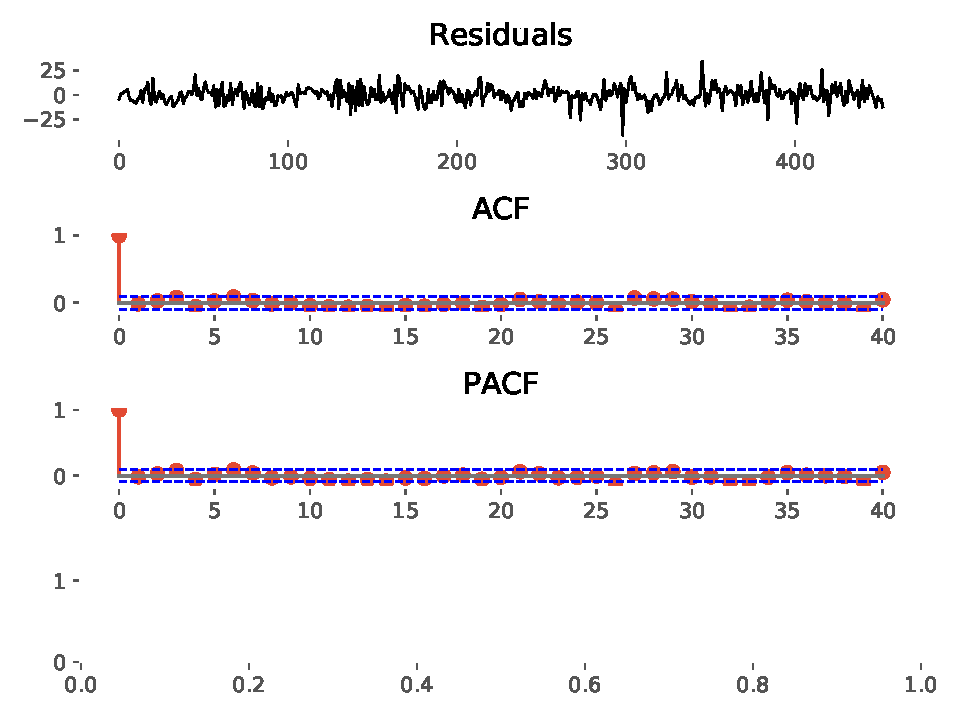
\includegraphics[width=0.70\textwidth]{task_2a.pdf}
        \caption{Plot av ACF og PACF av residualene.}
        \label{task_2a}
    \par}
    \end{figure}






\section{Oppgave 3}
\subsection{a-b)}

Prediksjon har blitt gjort med statsmodels sin ARMA-predict funksjon i python. Resultatet med 12 steg prediksjon er vist i figure(\ref{task_3}). Feilen konvergerer veldig fort til variansen av tidsrekken $\sigma_{x}$ som vist i figur(\ref{task_33}). Man kan også observere at prediksjonen konvergerer mot gjennomsnittet av tidsrekken.


\begin{figure}[hbt!]
    {\centering
        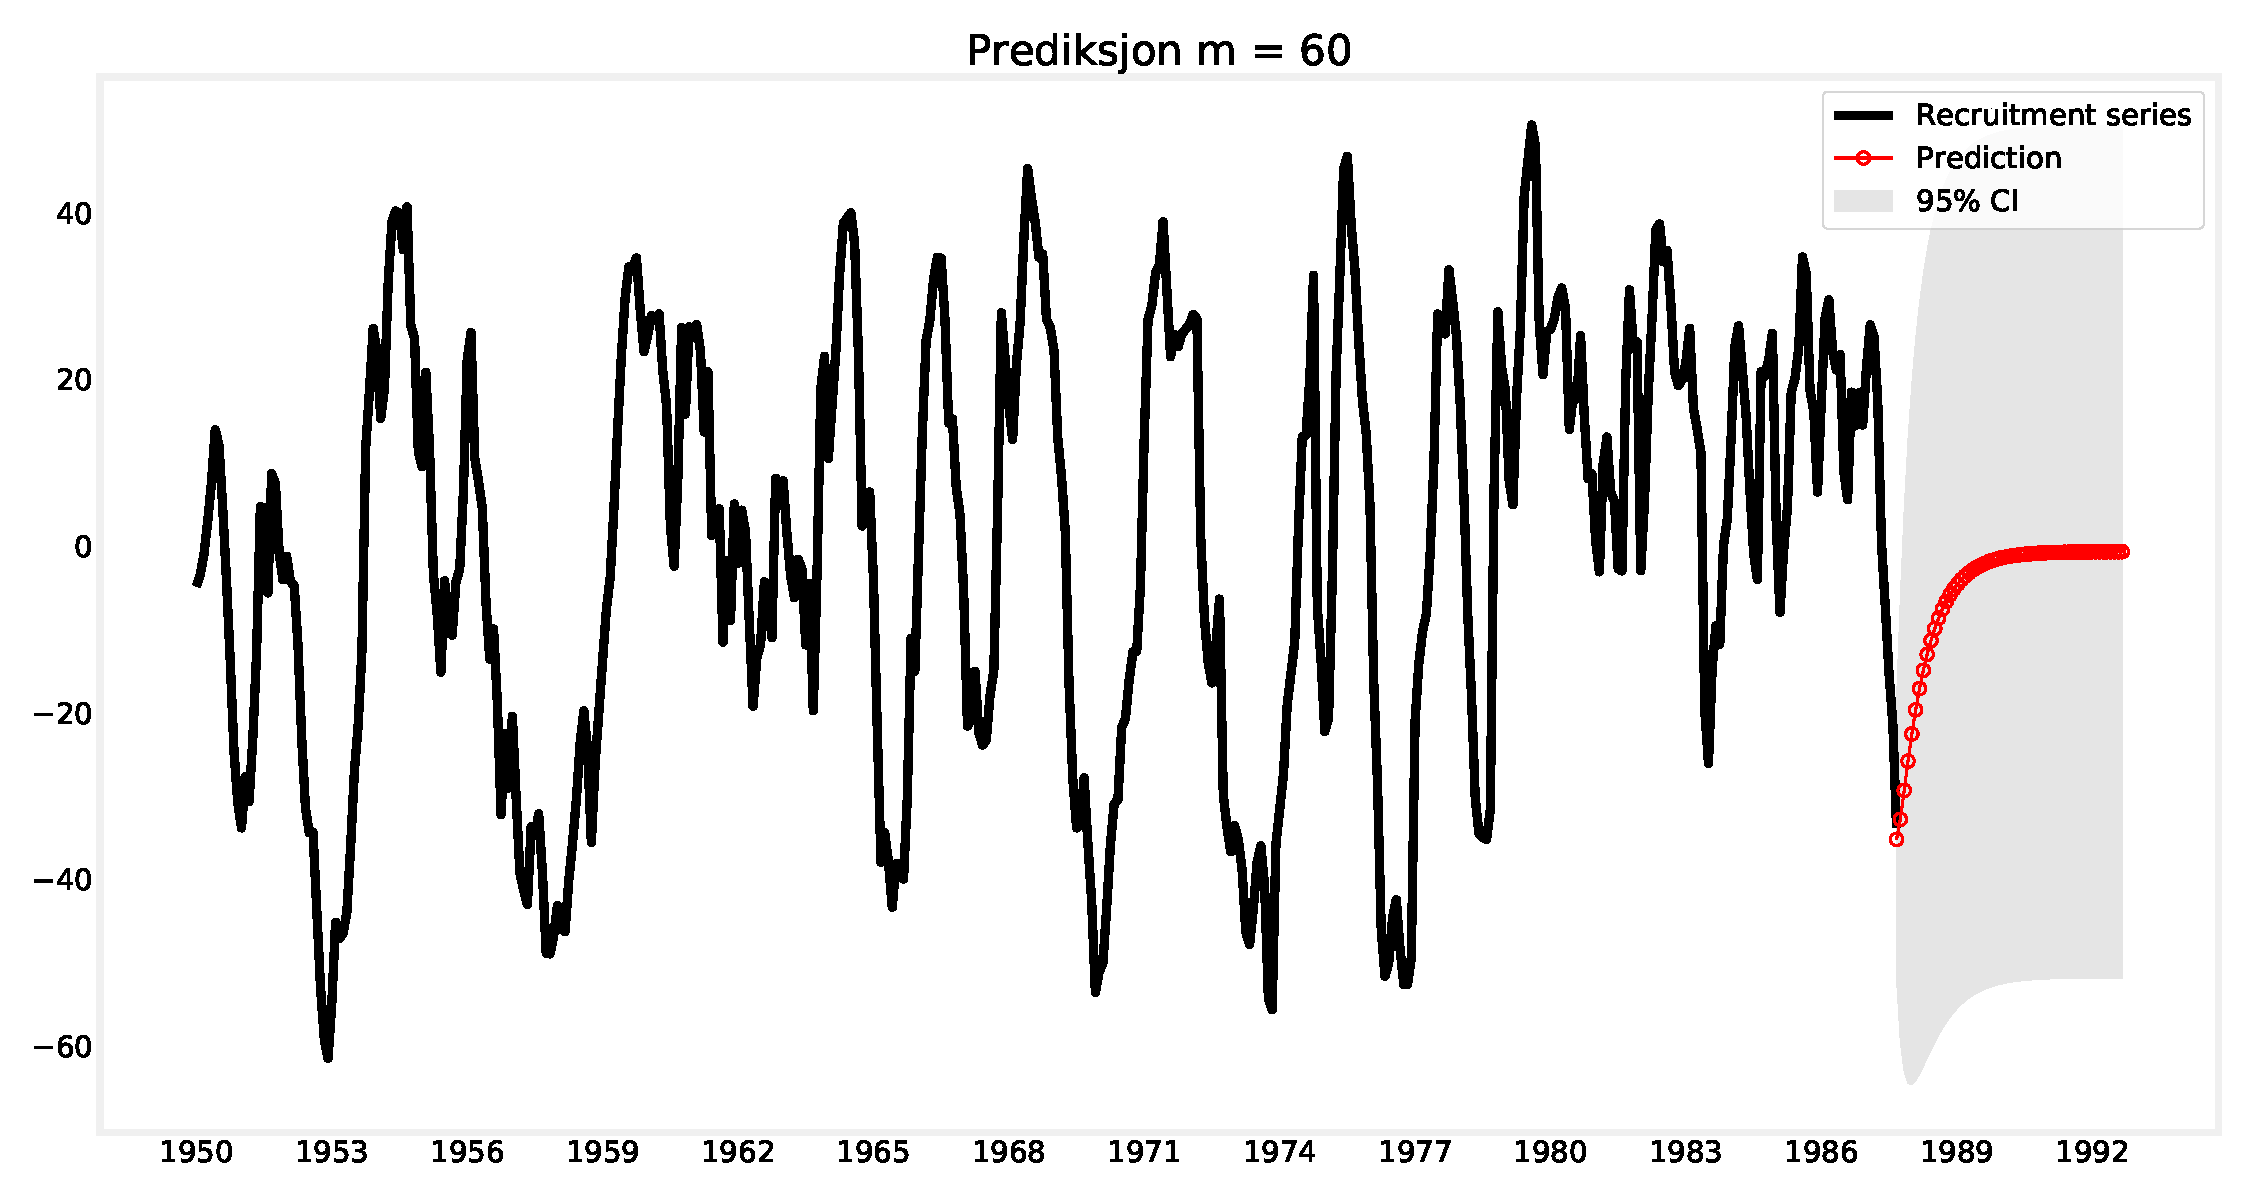
\includegraphics[width=0.80\textwidth]{task_33.pdf}
        \caption{Prediksjon med M = 12 måneder.}
        \label{task_3}
    \par}
    \end{figure}

    \begin{figure}[hbt!]
        {\centering
            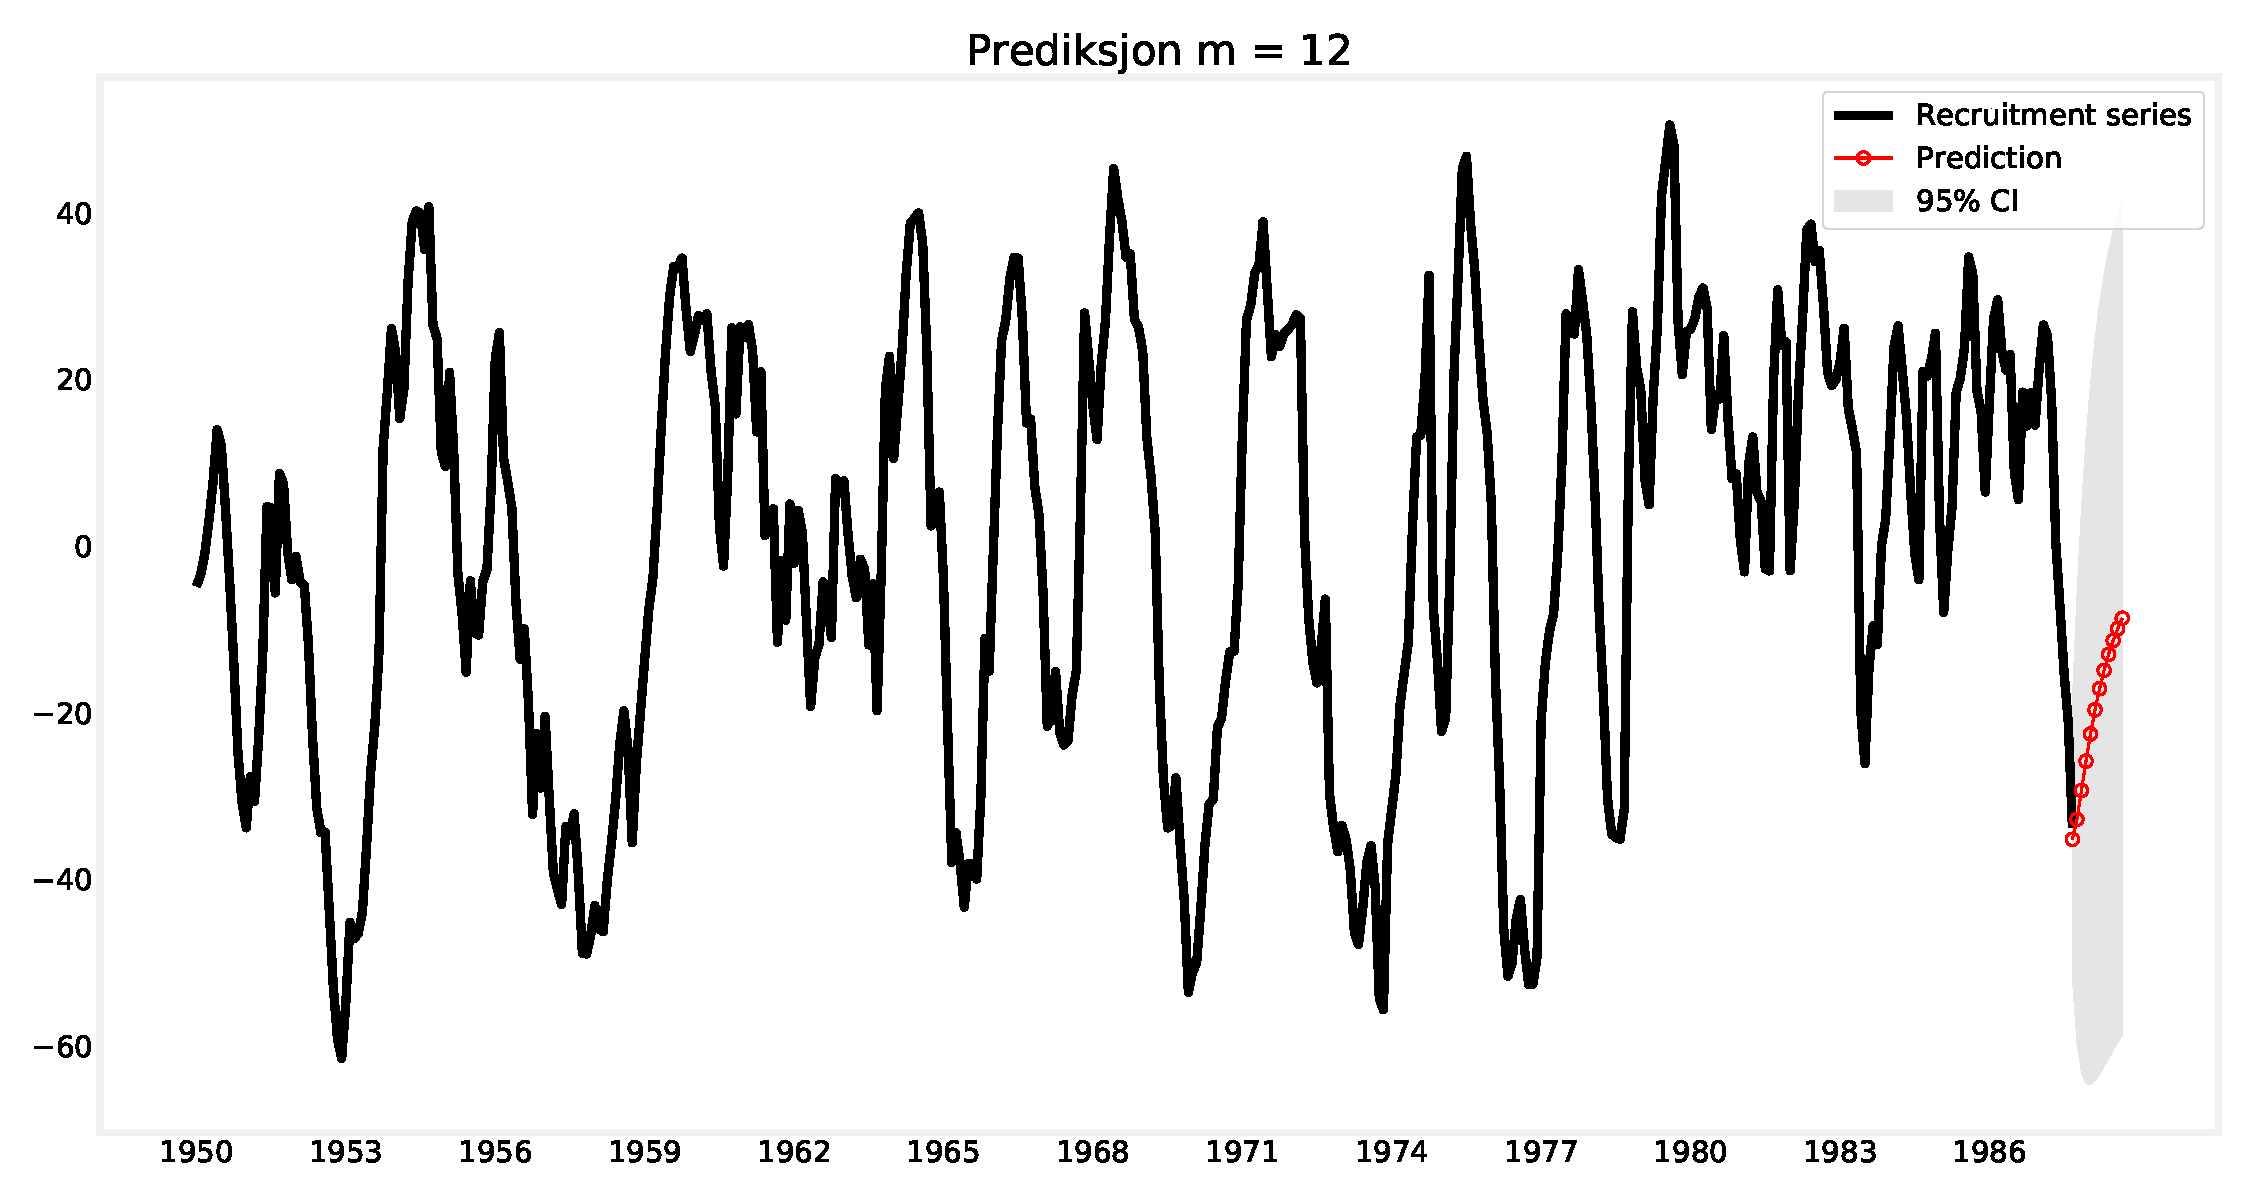
\includegraphics[width=0.80\textwidth]{task_3.pdf}
            \caption{Prediksjon med M = 60 måneder. Her kan man se at feilen konvergerer mot variansen til tidsserien når man bruker høy m.}
            \label{task_33}
        \par}
        \end{figure}











% --------------------------------------------------------------
%     Reference og appendix
% --------------------------------------------------------------
\clearpage
\newpage

\section{Appendix}


\begin{figure}[hbt!]
    \begin{lstlisting}

        from statsmodels.tsa.stattools import acf, pacf, ccf
        from statsmodels.tsa.arima_process import arma2ma, arma2ar
        import numpy as np
        import matplotlib.pyplot as plt
        import pandas as pd
        import os
        import statsmodels as sm
        plt.style.use('fivethirtyeight')
        plt.rcParams['axes.facecolor']='white'
        plt.rcParams['savefig.facecolor']='white'
        plt.rcParams['axes.grid']='off'
        
        # Load data
        rec = pd.read_csv('data/rec.txt', delimiter='\t')
        rec_df = pd.DataFrame(rec)
        time = np.copy(rec_df['year'])
        X = np.copy(rec_df['recruitment'])
    \end{lstlisting}
\caption{Load files}
\label{Kode2}
\end{figure}

\begin{figure}[hbt!]
    \begin{lstlisting}
        def w_periodogram(x, dt = 1):
        """Windowed periodogram"""
        #x = np.pad(x, (0,300), 'constant')
        N = len(x)
        n = np.arange(0,N,1)
        # Hann window
        window = (1/2)*(1 - np.cos(2*np.pi*n/(N-1)))
        U = (1/N)*np.sum(window**2)
        spectrum = np.abs(np.fft.fftshift(np.fft.fft(window*x)))**2
        spectrum *= (dt/(N*U))
        freq = np.fft.fftshift(np.fft.fftfreq(N, dt))
    
        return freq[int(N/2):], spectrum[int(N/2):]
    
    # Task A
    
    # Find periodogram
    freq, periodogram_X = w_periodogram(X)
    
    
    # Plot data
    fig, ax = plt.subplots(2,1)
    ax[0].plot(time, X, color = 'black')
    ax[0].set_title('Recruitment series')
    ax[0].set_xlabel('Year')
    ax[0].set_ylabel('Recruitment')
    ax[1].plot(freq[2:]*12, periodogram_X[2:], color = 'black')
    ax[1].set_title('Periodogram(hann windowed)')
    ax[1].set_xlabel('Frequency $\Delta f =$ year')
    ax[1].set_ylabel('Power')
    ax[1].set_xticks([x for x in np.arange(0, 6.5, 1/2)])
    plt.tight_layout()
    plt.savefig('rapport/task_a.pdf')
    plt.show()
    
    # Task B

    def remove_season(x):
        C = np.zeros(12)
        for m in range(0,12):
            C[m] = np.mean(x[m::12])
    
        # repeat C to create a periodic signal of equal length or longer than the dataset
        repC = np.tile(C, int(np.ceil(len(x)/12)))
        # compute residual (by subtracting periodic signal)
        X = x - repC[:len(x)]
        return X
    
    # Make stationary
    X_remseason = remove_season(X)
    
    plt.plot(time, X_remseason, color = 'black')
    plt.title('Recruitment series.')
    plt.tight_layout()
    plt.savefig('rapport/task_b.pdf')
    plt.show()
    
    # TASK C
    
    # make whitenoise Confidens intervall
    wt_line = 2*np.tile(1/np.sqrt(len(X_remseason)), 41)
    

    # Plot
    fig, ax = plt.subplots(2,1)
    # ax[0].plot(time, X_remseason)
    # ax[0].set_title('Stasjonre tidsserien')
    ax[0].stem(acf(X_remseason))
    ax[0].set_title('ACF')
    ax[0].plot(wt_line, '--', color = 'red', linewidth = 1); ax[0].plot(-wt_line, '--', color = 'red', linewidth = 1)
    ax[1].stem(pacf(X_remseason))
    ax[1].set_title('PACF')
    ax[1].plot(wt_line, '--', color = 'red', linewidth = 1); ax[1].plot(-wt_line, '--', color = 'red', linewidth = 1)
    plt.tight_layout()
    plt.savefig('rapport/task_c.pdf')
    plt.show()
    
    
    # Task D
    
    # Create model.
    model = sm.tsa.arima_model.ARIMA(X_remseason, order=(2, 0, 0))
    model_fit = model.fit()
    
    # Print result
    print(model_fit.summary())
\end{lstlisting}
\caption{Task 1}
\label{Kode3}
\end{figure}




\begin{figure}[hbt!]
    \begin{lstlisting}
        # Oppgave 2


        # Task A

        # Create model.
        model = sm.tsa.arima_model.ARIMA(X_remseason, order=(2, 0, 0))
        model_fit = model.fit()

        # Get residuals
        res = model_fit.resid
        
        # Plot
        fig, ax = plt.subplots(3,1)
        ax[0].plot(res, color = 'black')
        ax[0].set_title('Residuals')
        ax[1].stem(acf(res))
        ax[1].plot(wt_line, '--', color = 'red', linewidth = 1); ax[1].plot(-wt_line, '--', color = 'red', linewidth = 1)
        ax[1].set_title('ACF')
        ax[2].stem(pacf(res))
        ax[2].plot(wt_line, '--', color = 'red', linewidth = 1); ax[2].plot(-wt_line, '--', color = 'red', linewidth = 1)
        ax[2].set_title('PACF')
        plt.tight_layout()
        plt.savefig('rapport/task_2a.pdf')
        plt.show()
    \end{lstlisting}
\caption{Task 2}
\label{Kode4}
\end{figure}


\begin{figure}[hbt!]
    \begin{lstlisting}
        # Oppgave 3


        # Task A
        
        year = 5
        M = 12*year # 12*2 months (2 years)
        forecast, stderr, conf_int = model_fit.forecast(steps = M)
        # Default: 95% konfidensintervall
        
        
        sliced_time = time
        sliced_X = X_remseason
        time_forecast = np.linspace(sliced_time[-1], sliced_time[-1] + M/12, M)
        
        # Plot
        plt.figure(figsize = [15,8])
        plt.plot(sliced_time, sliced_X, color = 'black', label = 'Recruitment series')
        plt.plot(time_forecast, forecast, '-o', mfc='none', color = 'red', linewidth = '1', label = 'Prediction' )
        plt.fill_between(time_forecast, conf_int[:,0], conf_int[:,1], facecolor = (0, 0, 1, 0.2), label = '95% CI')
        plt.xticks([x for x in np.arange(sliced_time[0], sliced_time[-1]+ M/12, 3)])
        plt.legend(loc = 'best')
        plt.title('Prediksjon m = %s'%M)
        plt.tight_layout()
        plt.savefig('rapport/task_33.pdf')
        plt.show()
        
    \end{lstlisting}
\caption{Task 3}
\label{Kode5}
\end{figure}







\section{Referanser}
\begingroup
\renewcommand{\section}[2]{}%
%\renewcommand{\chapter}[2]{}% for other classes
\bibliographystyle{plainnat}
\bibliography{bibl}
\endgroup



% --------------------------------------------------------------
%     You don't have to mess with anything below this line.
% --------------------------------------------------------------
 





\end{document}


